% !TeX root = ./4-handout.tex

%possible excursion topics:
%bernadette's paradox, which i find puzzling, and relate briefly to causal explN; seems to me like Rayo and Yablo disagree about proper interpretation of this paradox! 
%causal explN background: e.g. woodward view (could be relevant for time-travel stuff, so could also save for later)
%rationality: straightforwardly factual vs. normative/plan-laden; defs relevant for decision theory unit!
%stuff on axiom of choice: relevant for bacon's puzzle
%could also save bacon puzzle for AoC unit! or return to later 
%could couple w/ Yablo's extension case, where the strategy to Bacon's paradox seems to lead to a genuine contradiction!!! see my notes in 3-thoughts and also the slides he sent me. Bevs vs. Owls 

% %Note to Josh if using these slides in a philsci class: I have some additional slides on phenomenology of eternalism, based on Spinrad's the weed of time short sci-fi story. could be fun to talk about in a longer unit on philosophy of time. see slides week 6 of my PHIL 154 sci-fi class! 


% They could incorporate/do if needing to kill time:
% chalk and talk the review sheet for this week
% talk about the strangeness of reductio proofs (could do this in future as well!); but defs relevant this week given large number of reductio proofs on the pset 
%changes to notion of rigor in mathematics; e.g. bolzano moving away from physical intuition , motion, passage of time. 


%\newcounter{mysection}
%\setcounter{mysection}{1}
%\arabic{mysection}
%\roman{subsection}

%\begin{itemize}[<+->] 
%\item<2-> % reveals second and keeps on page in subsequent frames
%\begin{itemize}[<2->] %does for a whole list of items


\setcounter{section}{3} %sets section counter to 0. note that need to switch section counter from Roman to arabic for this to work! since no roman numeral for 0! %put this into preamble, i.e. file common.tex: \renewcommand\thesection{\arabic{section}}




\section{Time Travel}
%\subsection*{test}

\begin{frame}
%\large

\scriptsize{\tableofcontents}

\end{frame}


\begin{frame}
\frametitle{Liable to forget:}
%\large

\begin{itemize}[<+->]

\item PSet 4 has been posted! Due this Sunday 3/19, 5pm!

\item[] questions 2--7 can be read in Part I quiz component

\item[] -- ideally, type answers to Part II :D 

\item Happy $\pi$-day!!! AMS booksale!!! 

\item Feel free to join \href{https://piazza.com/mit/spring2023/24118}{Piazza}! 

\item Feel free to join PSet partners!!! 
\item[] Groups will be auto-assigned Friday


\end{itemize}
\end{frame}

\subsection{Who's got the Time?}

\begin{frame}
\frametitle{Augustine Says}
%\large

I have a confession to make:

\pause 
\begin{quote}
Quid est ergo tempus? si nemo ex me quaerat scio; \\ si quarenti explicare velim, nescio. \\
\pause -- Saint Augustine in \textit{Confessions} XI.14 (year 354--430)
\end{quote}

\begin{itemize}[<+->]

\item Wittgenstein: ``This could not be said about a question of natural science. Something that one knows when nobody asks one, but no longer knows when one is asked to explain it, is something that has to be \textit{called to mind}''
\item[] ``And it is obviously something which, for some reason, it is difficult to call to mind''  -- \textit{Philosophical Investigations}, \S 89 

%and Witt goes on to discuss how this shows we are really interested in the CONCEPT of time, which concerns logical possibility or grammar, rather than physical possibility 

\end{itemize}

\end{frame}

\begin{frame}
\frametitle{And Wittgenstein Answers (\S 90)}
%\large

Recall our distinction between physical and logical possibility:

\begin{itemize}[<+->]

\item ``We feel as if we had to \textit{see right into} phenomena: yet our investigation is directed not towards \textit{phenomena}, but rather, as one might say, towards the `\textit{possibilities}' of phenomena.''

\item ``What that means is that we call to mind the \textit{kinds of statements} that we make about phenomena. So too, Augustine calls to mind the different statements that are made about the duration of events, about their being past, present or future. 
\item[] (These are, of course, not \textit{philosophical} statements about time, the past, the present and the future).''

\item ``Our inquiry is therefore a \emph{grammatical} one. And this inquiry sheds light on our problem by clearing misunderstandings away.''

\end{itemize}
\end{frame}

\iffalse

\begin{frame}
\frametitle{And Wittgenstein Answers (\S 90)}
%\large

Recall our distinction between physical and logical possibility:

\pause

\begin{quote}
-- We feel as if we had to \textit{see right into} phenomena: yet our investigation is directed not towards \textit{phenomena}, but rather, as one might say, towards the `\textit{possibilities}' of phenomena.
\end{quote}
\pause 
\begin{quote}
-- What that means is that we call to mind the kinds of statements that we make about phenomena. So too, Augustine calls to mind the different statements that are made about the duration of events, about their being past, present or future. (These are, of course, not philosophical statements about time, the past, the present and the future).
\end{quote}

% ``What that means is that we call to mind the kinds of statements that we make about phenomena. So too, Augustine calls to mind the different statements that are made about the duration of events, about their being past, present or future. (These are, of course, not philosophical statements about time, the past, the present and the future)''

%i.e. engaged statements rather than detached ones

\pause 

\begin{quote}
-- Our inquiry is therefore a grammatical one. And this inquiry sheds light on our problem by clearing misunderstandings away.
\end{quote}
\end{frame}

\fi 

\begin{frame}
\frametitle{Some Timely Questions}
%\large

\begin{enumerate}[<+->]

\item Is the past fixed while the future is open (i.e. not yet settled)?

\item Is the present in some sense more real than the past or future?

\item Is the passage of time real or an illusion? Does time really flow?

\item Does our perception of time give us knowledge of the nature of time?


\end{enumerate}
\end{frame}

\subsection{Time for Commonsense?}

\begin{frame}
\frametitle{A commonsense view about the past vs. the future }
%\large

\begin{itemize}[<+->]

\item The past is closed/fixed: the way the past was is settled
\item[] -- everything in the past has already happened, and that’s that

\item The future is open: it is not settled now the way the future will be
\item[] -- events in the future have not already happened
\item[] -- There is no fact about the way the future will be. 
\item[] -- There are many open possibilities.

\item \textbf{The past}: what has already happened and no longer exists
\item \emphz{The present}: what is happening now and is real (exists)
\item \emph{The future}: what has not yet happened and is not real yet

\item \textit{Question}: but is this merely how things seem to us?



\end{itemize}
\end{frame}




\begin{frame}
\frametitle{A commonsense view about time}
%\large

\begin{enumerate}[<+->]

\item \textit{Past vs. future}: the past is closed whereas the future is open.

\item \textit{Objectivity}: time’s passage is objective: it is independent of perspective and cannot be altered or controlled.

\item \textit{Epistemological asymmetry}: we can have extensive knowledge of the past and present, but it is impossible to have equally extensive knowledge of the future.

\item \textit{Ontological asymmetry}: things in the past used to exist but no longer do. Only the present currently exists. Future events have yet to exist.

\end{enumerate}
\pause 
Evidence for commonsense: this is how things na\"ively seem to us 

\end{frame}

\begin{frame}
\frametitle{A commonsense view of the passage of time}
%\large

\begin{itemize}%skip this slide![<+->]

\item Time’s passage: our experiences go from past to future
\item[] -- based always in the present
\item[] -- the present fades into the past as we move toward the future

\item Passage of time is objective or absolute: time passes the same for everyone, independently of their perspective

\item Question: is the passage of time real? 
\item[] -- Or, is it simply an artifact of our human psychology? 
\item[] -- Or an artifact of our epistemic situation? Memories?

\item Analogy: we used to think the Earth was at the center of the universe, simply because that is how things seemed to us. 



\end{itemize}
\end{frame}

\subsection{Presentism vs. Eternalism}

\begin{frame}
\frametitle{The ontology of time: presentism vs. eternalism}
%\large

\begin{itemize}[<+->]

\item It is orienting to consider two ontologies at opposite extremes

\item \emphz{DISCLAIMER}: Eternalism will be the VIEW TO REMEMBER here

\item We'll talk a bit about presentism, but DO NOT appeal to it in the problem set. It will at best lead you astray

\item TL;DR: The present is a cruel mistress 


\end{itemize}
\end{frame}


\begin{frame}
\frametitle{Presentism (here for a short time, not a long time!)}
%\large

%thing to flag: time travel would seemingly be logically impossible if presentism is true: how could you travel somewhere that doesn't exist!? 

%burn after reading; going going gone; only for the here and now 
\begin{columns}
    \begin{column}{.6\textwidth}
\begin{itemize}[<+->]

\item Only events in the present exist
\item Events in the past existed, but do not now exist
\item Present events are more real than past or future events
\item Passage of time is real
\end{itemize}
  \end{column}
 
    \begin{column}{.4\textwidth}  
 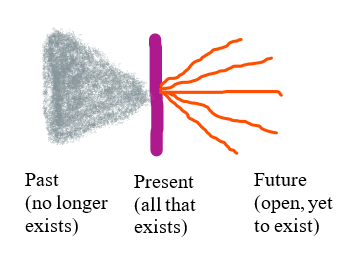
\includegraphics[height=.6\textheight]{../assets/presentism}
 
   \pause remember: \textit{burn after reading}

    \end{column}
  \end{columns}
  

\end{frame}

\begin{frame}
\frametitle{Eternalism (it will never leave you)}
%\large

%burn after reading; going going gone; only for the here and now 
\begin{columns}
    \begin{column}{.55\textwidth}
\begin{itemize}[<+->]

\item All events in the past, present, and future exist
\item These events are equally real \\ (no ontological asymmetries)
\item Abraham Lincoln is just as real as Barack Obama
\item[] (but not as baller, obviously) 
\item Existence includes everything that has existed, is existing, and will exist. Existence is eternal
\item Passage of time is an illusion 

\end{itemize}
  \end{column}
 
    \begin{column}{.45\textwidth}  
 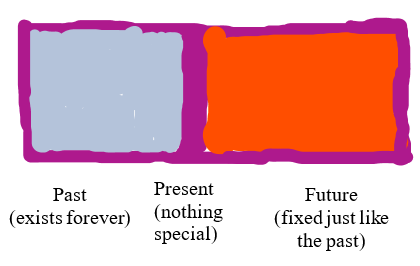
\includegraphics[height=.6\textheight]{../assets/eternalism}
 
   \pause (so if it seems like this class will never end\dots)

    \end{column}
  \end{columns}
  

\end{frame}

\begin{frame}
\frametitle{Phil Prompt \#9 (just in time!)}
%\large

\begin{itemize}[<+->]

\item Which do you find more plausible: presentism or eternalism?

\item Is the passage of time an illusion? 

\item Can you think of a more compelling ontology for time?

\item Optional bonus: What \textit{is} time? 

\end{itemize}
\end{frame}

\begin{frame}
\frametitle{Eternalism: analogy with space}
%\large

\begin{itemize}[<+->]

\item We think that all places on Earth are equally real 
\item[] -- not just the place that is here
\item Spatial locations constitute a fixed 3-dimensional “block”:  latitude, longitude, height
\item[] -- Google Earth view: can see the whole 3-dimensional block

\item Eternalist: different space-time events analogous to different spatial positions: all just as real (not only the time that is now)
\item[] -- All timelessly coexist, albeit they occupy different times 
\item Universe $=$ fixed 4-dimensional block (3 space dims + time)
\item[] -- God’s eye view: can see the whole block
\item Differences between past, present, and future are perspectival

\end{itemize}
\end{frame}

\begin{frame}
\frametitle{On the (eternal non-) passage of time}
%\large

\begin{itemize}%[<+->] %skip slide and head to determinism! 

\item Intuitively, time passes only if things change
\item If nothing changes, then time does not pass


\item[] [Ney 2014, 152]: ``the passage of time is precisely a change in which objects and events exist. It is old (past) objects and events passing out of existence and new (what were future) objects and events coming to be'' 

\item Eternalism: incompatible with temporal passage b/c no change
\bi
\item everything is fixed from time immemorial
\item so, the passage of time is an illusion
\item Merely part of our phenomenology or epistemic situation
\ei
\item So it would be physically possible that beings different from us could experience time differently or that we could alter how we perceive time %drugs anyone? 
% could change your perception of time


\end{itemize}
\end{frame}




\iffalse
\begin{quote}
the passage of time is precisely a change in which objects and events exist. It is old (past) objects and events passing out of existence and new (what were future) objects and events coming to be. [Ney 2014, 152]
\end{quote}
\fi 


% %Note to Josh if using these slides in a philsci class: I have some additional slides on phenomenology of eternalism, based on Spinrad's the weed of time short sci-fi story. could be fun to talk about in a longer unit on philosophy of time. see slides week 6 of my PHIL 154 sci-fi class! 

\subsection{Determinism}

\begin{frame}
\frametitle{Determinism!}
%\large

\begin{itemize}[<+->]

\item \textbf{Deterministic evolution}: given (i) the laws and (ii) complete information about a state (e.g. initial and boundary conditions), all \textit{future} states are uniquely determined 

\item \textit{Reversibility}: given (i) and (ii), all \textit{past} states are determined  

\item \emph{Determinism}: the universe evolves deterministically 
% Or more modestly: everything within your light cone, since that's all that matters for you. modulo entanglement

% Of course, if the laws are time reversible, then determinism entails reversibility. 

\item \emphz{Indeterminism}: the past does not determine the future 

\item Note well: determinism entails that the future is fixed/settled, but the claim that $\langle$the future is settled$\rangle$ does NOT entail determinism

\item For instance, eternalism does not entail determinism. 
\item[] -- The future could be settled without the future being determined by past events plus laws.

\end{itemize}
\end{frame}

\begin{frame}
\frametitle{Determinism is NOT \emphz{Fatalism}!}
%\large

\begin{itemize}[<+->]

\item CRUCIAL: distinguish determinism from \emphz{fatalism}: whatever happens in the future is going to happen \textit{no matter what we do}

\item e.g. fatalism about climate catastrophe: \\ no matter what we do, the ice-caps will melt soon 
%we are doomed
%e.g., a fatalist about climate change would say that no matter how much we try to prevent/slowdown climate change, its disastrous effects are inevitable

\item[] -- Fatalism goes beyond determinism

\item It may be deterministically the case right now that we are doomed, but not that we're doomed no matter what we do. 

\item If fatalism is false, our actions, decisions, choices etc. still make a difference to the way the world is (even if we could not have chosen otherwise, e.g. because determinism is true)

% % Another example, which comes up on the problem set: it may be determined that you are going to do well on your exam. But it might still be the case that if you don't study, then you will fail. It's just also determinant that you are going to study.

\end{itemize}
\end{frame}

\subsection{Time Travel}

\begin{frame}
\frametitle{Two notions of `time'}
%\large

\begin{itemize}[<+->]

\item \emph{External time}: how much time has passed according to the world external to the time traveler (e.g. how much time has passed on earth)

\item \emphz{Personal time}: how much time has passed according to the time traveler.
\item[] -- How much time they experience passing (e.g. the duration of their trip)
\item[] -- How much time has passed according to their personal watch/clock
\item[] -- Or according to their biological processes, e.g. hair growth, digestion
%\item[] -- Also called “proper time”
\end{itemize}
\end{frame}

\begin{frame}
\frametitle{What is time travel anyway?}
%\large

\begin{itemize}[<+->]

\item Lewis: \textbf{time travel} occurs whenever there is a discrepancy between someone’s personal time and external time
%so twin's paradox involves time travel! 

\item Time-slide to the future: less personal time has passed than external time 
\item[] -- e.g., moving through a whole century in five minutes

\item Time-slide to the past: personal time has passed, but the external time is earlier
\item[] -- e.g., rewinding a whole century in five minutes


\end{itemize}
\end{frame}

\begin{frame}
\frametitle{Changing the Past (or future)?}
%\large

\begin{itemize}[<+->]

\item If we can time travel, can we change the past (or future)?

\item Assuming that eternalism is true, then no!
\item The past and future are fixed: the events there are settled, once and for all
\item Whatever happened in the past happened; you can’t change that
\item[] -- What happens in Vegas, stays in Vegas (in the past!)

\item[] \#I have no regrets 
%as uttered on my napkin for a croissant 

\end{itemize}
\end{frame}



\begin{frame}
\frametitle{The Logical Impossibility of Changing the Past}
%\large

\begin{itemize}[<+->]

\item Even if eternalism is false, changing the past involves a contradiction

\item Changing the past therefore seems logically impossible!

\item Argument: Grandfather's paradox (or more mundane cases)

\item e.g. it can't be both true that you drank exactly five glasses of water yesterday and true that you drank exactly eight glasses of water yesterday

\item if something is logically impossible, then it must be physically impossible as well

\end{itemize}
\end{frame}

\begin{frame}
\frametitle{Affecting the Past}
%\large

\begin{itemize}[<+->]

\item If we can time travel, can we \textit{affect} the past?

\item Yes! (in the sense that you could perform actions in the past)

\item Even if your actions are set in timeless stone, your actions still causally matter 
\item[] -- They still make a difference to the way the world is.
%\item Connection with compatibilism: even if all your future actions are determined, your future actions still affect the future (even if you can’t change them)
\item The impossibility of changing the past does not entail that you necessarily made no difference to the past. 
\item[] -- You might have time traveled and saved the world! 
%interesting wrinkle: if you have time-traveled to the past and done something important, you might not know that now. you might only find out later! 

\end{itemize}
\end{frame}

\begin{frame}
\frametitle{Affecting vs. Changing the Past}
%\large

\begin{itemize}[<+->]

\item Lewis (p. 5): you can make the past (or future) different from what it \textit{would have been otherwise} without the action you performed

\item[] -- Notice that this subjunctive conditional does NOT entail that you could have acted otherwise

\item[] -- This is not changing the past (or future): it is affecting it

\item This notion of affecting (but not changing) the past is closely connected to a notion of free will that is compatible with determinism
%if you had wanted to, you could have acted differently


\end{itemize}
\end{frame}

\begin{frame}
\frametitle{Two Notions of Capacity or Freedom}
%\large

\begin{itemize}[<+->]

\item In what sense, if any, can you kill your grandfather in an external time before you were born?

\item Lewis: two different notions of “can”. Don’t equivocate b/w them!

\item Can$_{capacity/skill}$: having the skill or ability it takes to do something
\item[] -- Lewis: by training with a rifle, etc. you could gain the capacity
\item[] -- You could have what it takes (mentally, physically, etc.)
%o	In this sense, you couldskill kill your past self

\item Can$_{logic}$: ability to do something without it resulting in a logical contradiction
\item[] -- No matter what, you know that you must fail in killing your gF
\item[] -- For you know that you lived to travel back in time
\item[] -- And it can’t be both true and false that you were born
\item[] -- So you logically can’t kill your grandfather
\item[] -- But failing does not entail that you couldn’t$_{capacity/skill}$ do it

\end{itemize}
\end{frame}

\begin{frame}
\frametitle{So what would happen if you tried?}
%\large

\begin{itemize}[<+->]

\item What would stop you? Coincidences? Mundane contingencies?

\item Do the laws of logic function as meta-laws constraining physical reality/physical laws?

\end{itemize}
\end{frame}

\begin{frame}
\frametitle{Philosophy Prompt \#10}
%\large

\begin{itemize}[<+->]

\item Imagine that you time travel to 1940 and that you can$_{capacity}$ kill your grandfather.

\item[1.] Is there a satisfying explanation as to why you fail? 

\item[] -- What, if anything, is dissatisfying about a detailed causal-mechanical story of what happens? 

\item[2.] Now imagine that we ALL can$_{capacity}$ do this. Is there a satisfying explanation for the following fact: \\ $\langle$Everyone in 24.118 fails to kill their grandfathers$\rangle$

%e.g. is it satisfying to explain a conjunction of events by conjoining individual causal-mechanical explNs. is there a unified explN? 

\item[] (\textit{Disclaimer}: no actual grandparents were harmed in the construction of this thought experiment)
\item[] \#Cherish your grandparents

%Idea: no unified explN. 
\end{itemize}
\end{frame}

\subsection{Closed Causal Loops}

\begin{frame}
\frametitle{Closed Causal Loops}
%\large

\begin{itemize}[<+->]


\item Three events occur sequentially in external time: A, B, and C
\item[] -- A causes B and B causes C (so far so good! This is normal)
\item[] -- But now, C causes A (reverse causation); thanks to time travel
\item If this were true, then causes would not always precede their effects
\item very strange! But not impossible! At least not logically

\end{itemize}
\end{frame}

\begin{frame}
\frametitle{Illustrating Causal Loops}
%\large

\begin{itemize}[<+->]

\item At 20 years old, you learn how to build a time machine (A) \\ (we’ll consider how below!)
\item Using this knowledge, you build one and record detailed instructions (A → B)
\item From these records, your 40-year-old self knows how to build a time machine (B → C)
\item Using the Time Machine, you travel back in time and talk to your 20-year-old self. 
\item[] -- You tell them how to build a time machine (C → A)
\item[] -- This is how you at 20 years old learned how to build one % in the first place
\item \textit{Puzzle}: where did the knowledge come from ``originally''? 
\item[] -- Is there any causal-mechanical explanation of it??? 

\end{itemize}
\end{frame}

\begin{frame}
\frametitle{Lewis on Causal Loops}
%\large

\begin{itemize}[<+->]

\item Every event in this sequence has a cause and therefore an explanation
\item But the entire causal loop itself does not have an explanation
\item There is ``simply no answer'' to the question of where the relevant knowledge or information came from, or even why any of this took place (page 4).
\item So we can explain the individual parts, even as we cannot explain the whole loop itself!


\end{itemize}
\end{frame}



\begin{frame}
\frametitle{A Problem for Eternalism?}
%\large

\begin{itemize}%[<+->]

\item Is the difficulty or absence of time-travel a problem for eternalism?
\item Recall that eternalism puts time on the same footing as space
\item We have a really easy time moving around space (provided we don’t bump into things)
\item Why do we have such a hard time moving around time?! %is there `something we're always bumping into temporally???'
\item It appears as though we are condemned to only move into the future, never into the past
\item But if the past and future are really on the same ontological footing, why do we only ever move into the future?
\item Likewise, if the passage of time is really an illusion, why can’t we visit the past?
%•	One eternalist response: time travel is possible. It’s just really hard! Thus really rare!

\end{itemize}
\end{frame}


\iffalse 


\subsection{Free Willy!}

\begin{frame}
\frametitle{Surface Free Will (just superficial enough)}
%\large

\begin{itemize}[<+->]

\item \emph{Surface free will} (a.k.a. compatibilist free will or political free will): the political or social ability to make choices that satisfy your desires. The freedom to do what you want to do.
\item Perhaps the ordinary or intuitive notion of freedom of choice/will
\item A power or ability to choose something rather than something else
\item ``unconstrained freedom of choice or decision'' [Kane, p. 15], \\ coming from within you

\item as in, \textit{Reach for the stars, not drugs} 

\end{itemize}
\end{frame}

\begin{frame}
\frametitle{Libertarian Free Will (it's apolitical!)}
%\large

\begin{itemize}[<+->]

\item \emphz{Libertarian Free Will}: (a.k.a.` free will of origination'): 
\item[] -- the ability to choose what you \textit{want to want} or want to desire. 
\item Having ultimate power over what you will/want/desire. %Kane refers to this as a deeper sense of free will
\item ``a kind of ultimate control over what you will or want in the first place'' [Kane, p. 15]

\item The kind of free will your soul craves 


\end{itemize}
\end{frame}

\begin{frame}
\frametitle{Compatibilism vs. Incompatibilism}
%\large

\begin{itemize}[<+->]

\item \textbf{Compatibility Question}: is free will compatible with determinism? Likewise, is free will compatible with any physically-plausible version of indeterminism?

\item If you answer `yes,' then you are a \emph{compatibilist}
\item[] -- \textit{soft determinist}: you also believe determinism is true 

\item If you answer `no,' then you are an \emphz{incompatibilist}: 

\item \textit{hard determinist}: you also believe that determinism is true
\item[] -- so you deny we have the relevant kind of free will

\item \textit{libertarian} (about free will): you also deny determinism
\item[] -- so you believe we do have free will (modulo worries about compatibility with indeterminism!)

\end{itemize}
\end{frame}

\begin{frame}
\frametitle{(Classical) Compatibilism}
%\large

\begin{itemize}[<+->]

%\item free will has one necessary and sufficient condition: 

\item (Classical) \emph{Compatibilism}: you acted freely if and only if you met the following condition: 

\item \textbf{Weak Principle of Alternative Possibilities}: if you had wanted to choose otherwise than you did, then nothing would have prevented you from choosing otherwise.
%Frankfurt cases provide a counterexample to the necessity of this condition. still seems sufficient though. 

\item Notice that meeting this condition entails that another claim holds: you have the power or ability to make a choice in the sense that nothing constrains you or prevents you from making that choice

\item According to compatibilism, a sufficient condition for LACKING free will in a given circumstance is that you are constrained, coerced, or otherwise manipulated


%\item Hence, if anything does constrain you or prevent you from making that choice, then you don’t have this power or ability to do what you want to do, and hence you could not have chosen otherwise. 

\end{itemize}
\end{frame}

\begin{frame}
\frametitle{Compatibility with Moral Responsibility}
%\large

\begin{itemize}[<+->]

\item Imagine that you don't think free will is necessary for moral responsibility: e.g. an agent can be morally responsible for their actions even if they did not act freely 
\item[] -- roughly, you think it would still be appropriate to praise or blame this agent for their action

\item You might then ask a similar `compatibility question' about whether moral responsibility is compatible with determinism

\item e.g. perhaps \textit{surface free will} suffices for moral responsibility 

\item When it comes to social and political decisions, you might think that moral responsibility is really what matters 

\end{itemize}
\end{frame}



\fi 


















